\documentclass[11pt]{article}
\title{\textbf{Microbiologia}}
\author{Simona Debilio}
\date{}

\usepackage{graphicx}
\usepackage[utf8x]{inputenc}
\usepackage[italian]{babel}
\setlength{\parindent}{0pt}

\begin{document}

\maketitle

\tableofcontents

\clearpage

\section{Struttura e funzione di una cellula procariote}

Con il termine \emph{``microrganismo''} si indicano organismi dalle dimensioni molto piccole che possono essere sia procarioti che eucarioti (lieviti, muffe, ecc...).
Questi due tipi cellulari condividono alcune caratteristiche:
\begin{itemize}
\item Tutte le cellule presentano una membrana plasmatica;
\item Il citoplasma ha una composizione simile;
\item Entrambe possiedono ribosomi (la composizione e il peso di quest'ultimi però variano tra le due).
\end{itemize}
\vspace{1em}
Caratteristiche distintive dei \emph{procarioti}:
\begin{itemize}
\item Sono organismi unicellulari;
\item La cellula procariote non ha organelli cellulari oltre ai ribosomi;
\item Non possiedono mitocondri, l'energia viene prodotta a livello della membrana cellulare;
\item Hanno maggiore semplicità strutturale e minori dimensioni della cellula;
\item La divisione cellulare avviene tramite la scissione binaria.
\end{itemize} 
\vspace{1em}
I procarioti si dividono in due grandi gruppi:
\begin{enumerate}
\item \textbf{Batteri};
\item \textbf{Archea}.
\end{enumerate}
\vspace{1em}
Nei batteri si trova un unico cromosoma circolare.
Avendo poco spazio all'interno della cellula, il 98\% del materiale genetico dei batteri è codificante (non sono presenti gli istoni).
\\Nei procarioti è possibile che ci sia del materiale genetico accessorio (come ad esempio i plasmidi) autoreplicante, cioè indipendente dal cromosoma per la sua replicazione, che apporta al batterio capacità accessorie (virulenza, resistenza alla salinità, resistenza gli antibiotici...).\\

La \textbf{parete cellulare} nei batteri è formata da \textbf{peptidoglicano} (mai presente negli eucarioti).
I batteri possiedono dei \textbf{flagelli} che gli permettono di muoversi: un batterio dotato di flagelli è molto più aggressivo perché è in grado di spostarsi in altre zone più adatte alla vita.
I batteri presentano anche dei \textbf{pili} (utilizzati nella coniugazione).\\

Il peptidoglicano è tipico della parete dei batteri, mentre gli Archea possiedono uno \textbf{pseudopeptidoglicano}.
A differenza dei batteri, gli Archea possono crescere a temperature superiori ai 100 gradi.\\

Le dimensioni standard della cellula batterica vanno dagli 0,2 ai 2 micron.
La cellula modello è quella di E. Coli.\\

Esistono delle dimensioni ottimali per il batterio: dimensioni piccole infatti consentono alla cellula di poter effetturare scambi più efficienti con l'esterno. Inoltre, le dimensioni influenzano il tasso di trasporto di nutrienti e prodotti di scarto del metabolismo attraverso la cellula.\\

Aumentando le dimensioni aumenta anche il rapporto tra la superficie ed il volule cellulare rendendo gli scambi con l'esterno meno efficienti.\\

I batteri possono essere suddivisi, in base della loro forma, in:
\begin{itemize}
\item \textbf{Cocchi}, dalla forma sferica;
\item \textbf{Bacilli}, dalla forma a bastoncino;
\item \textbf{Coccobacilli}, dalla forma intermedia tra cocchi e bacilli.
\end{itemize}
\clearpage
A seconda del tipo di divisione effettuata dai cocchi poi, si possono riconoscere:
\begin{itemize}
\item \textbf{Diplococchi} o \textbf{streptococchi}, se il cocco si divide secondo \emph{un} piano verticale;
\item \textbf{Tetradi}, se il cocco si divide secondo \emph{due} piani verticali e uno orizzontale;
\item \textbf{Sarcine}, se il cocco si divide secondo \emph{due piani verticali e uno orizzontale};
\item \textbf{Stafilococchi}, se i cocchi si dividono in maniera disordinata.
\end{itemize}

\vspace{1em}
Oppure possono assumere forme ricurve, e allora vengono suddivisi in:
\begin{itemize}
\item \textbf{Vibrione}, dalla forma a bastoncino leggermente ricurvo;
\item \textbf{Spirilli}, dalla forma più ricurva rispetto ai vibrioni;
\item \textbf{Spirocheti}, dalla forma quasi ad elica.
\end{itemize}
Ciò che cambia è la flessibilità del batterio: le spirochete sono più flessibili dei vibrioni.\\

Esistono poi altri due tipi di batteri:
\begin{itemize}
\item I \textbf{batteri prostecati}, i quali possiedono un peduncolo di adesione al substrato;
\item I \textbf{batteri filamentosi}, formati da ife e micelio.
\end{itemize}

\vspace{1em}
Dalla divisione cellulare del \emph{Caulobacter}, un batterio prostecato, si ottengono due cellule attaccate l'una all'altra di cui una presenta un peduncolo e l'altra presenta un flagello. \\Successivamente la cellula con il flagello si stacca e forma una cellula a parte.\\

I batteri presentano proteine simili a quelle del citoscheletro delle cellule eucarioti regolano la forma e la dimensione delle cellule batteriche durante l'accrescimento.
\\Ad esempio:
\begin{itemize}
\item \textbf{FtsZ}, nei cocchi, si concentra in posizione mediana e coordina la formaizone della nuova parete cellulare che separerà le due cellule;
\item \textbf{MreB}, nei bastoncelli, forma una struttura elicoidale a livello della membrana plasmatica;
\item \textbf{CreS} (detta "crescentina") è responsabile della curvatura della cellula.
\end{itemize}

\section{Il rivestimento della cellula batterica}

La cellula procariote presenta complesse strutture di rivestimento che consentono al batterio di adattarsi a condizioni ambientali anche estreme.

Tutte le cellule procariote presentano una membrana plasmatica che separa l'interno della cellula dall'esterno. 

In generale i batteri presentano anche una parete che ha composizione e posizione diversa a seconda del gruppo microbico.

Possono poi essere presenti altre strutture di rivestimento (strato S, capsula, glicocalice...) e appendici di superficie (pili e flagelli).

I batteri che presentano la capsula sono particolarmente virulenti perché protetti molto bene e dunque molto resistenti.

\subsection{Differenze nella composizione dell'involucro esterno tra batteri Gram+ e Gram-}
I batteri \textbf{Gram+} presentano (partendo dall'interno):
\begin{itemize}
\item Una membrana plasmatica a doppo strato fosfolipidico;
\item Un sottile strato detto periplasma in cui vengono riversati enzimi e in cui avvengono reazioni metaboliche;
\item Uno strato spesso di peptidoglicano.
\end{itemize}

I \textbf{Gram-} presentano (partendo dall'interno):
\begin{itemize}
\item una membrana plasmatica;
\item un periplasma spesso in cui è immerso un sottile strato di peptidoglicano;
\item una membrana esterna (diversa chimicamente dalla membrana plasmatica).
\end{itemize}

\begin{figure}[htp]
\centering
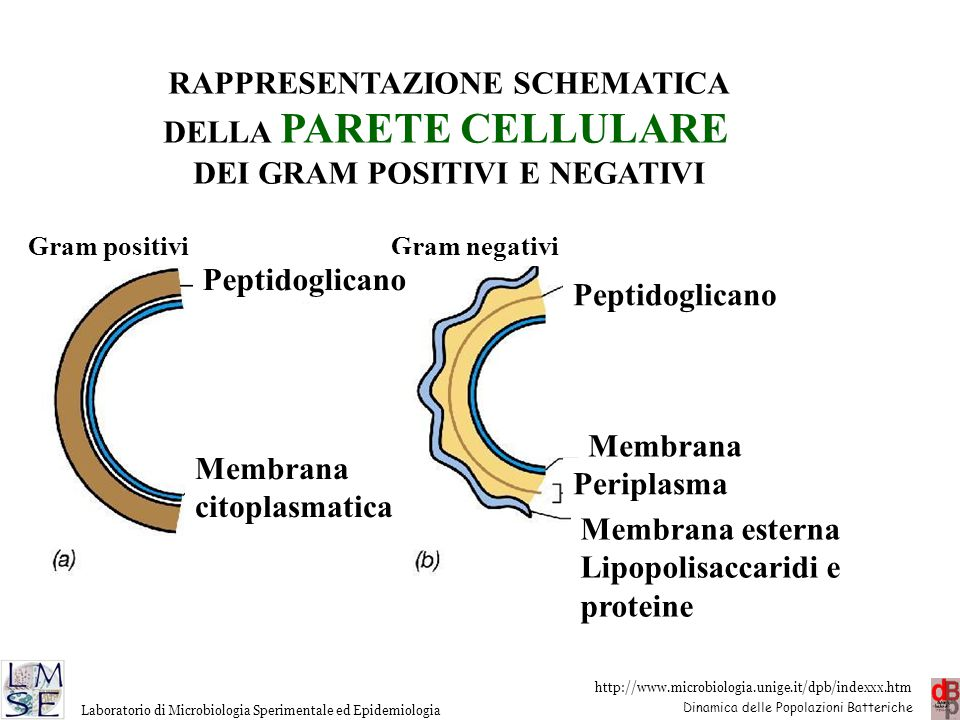
\includegraphics[scale=0.40]{img/parete_cellulare.jpg}
\caption{Differenze nella membrana tra batteri Gram+ e Gram-}
\label{parete_cellulare}
\end{figure}

\subsubsection{Composizione della membrana plasmatica}
Nei batteri la membrana plasmatica è formata da una membrana fosfolipidica classica: un doppio strato fosfolipidico organizzato con le teste polari rivolte verso l'esterno e le code idrofobiche rivolte verso l'interno.\\

Esistono tuttavia delle differenze nella composizione tra la membrana dei Bacteria e quella degli Archea.\\

Nei \textbf{Bacteria}:
\begin{itemize}
\item La \emph{testa} del fosfolipide è formata da una molecola di \textbf{D-glicerolo-3-fosfato}. Al fosfato esterificato al C3 possono essere legati dei gruppi funzionali;
\item La \emph{coda} è costituita da \textbf{due molecole di acidi grassi esterificati} al C1 e C2 (in maggioranza sono \textbf{saturi}, con aggiustamenti dettati da variazioni ambientali);
\item Il gruppo fosfato è esterificato sul \textbf{C3}.
\end{itemize}

\vspace{1em}
Tipicamente, nelle membrane dei Bacteria sono assenti gli steroli (con l'eccezione dei metilotrofi), come il colesterolo, i quali sono sostituiti dagli \textbf{opanoidi}.
Gli opanoidi contribuiscono a stabilizzare la struttura e a renderla meno flessibile (svolgono la stessa funzione del colesterolo nelle cellule eucariote).\\

Negli \textbf{Archea}:
\begin{itemize}
\item La testa del fosfolipide è formata da una molecola di \textbf{L-glicerolo-3-fosfato}. I legami con le catene idrofobiche si formano al C2 e al C3;
\item Negli Archea il legame tra il glicerolo e le catene alifatiche, ovvero le catene di acidi grassi, sono \textbf{eteri} (e NON esteri)
\item Il gruppo fosfato è esterificato sul \textbf{C1};
\item Negli Archea le catene di acidi grassi sono costituite da catene di \textbf{isoprene} contenenti doppi legami.
\end{itemize}

\vspace{1em}
I lipidi degli Archea possono essere \textbf{dieteri} (cioè con 2 catene alifatiche a 20C legate covalentemente al glicerolo) o \textbf{tetraeteri} (cioè 2 catene alifatiche a 40C legate a due molecole di glicerolo) del glicerolo. 

Negli Archea a volte non è presente un doppio strato fosfolipidico, ma un monostrato fosfolipidico il quale garantisce una maggiore stabilità alle membrane (si trova frequentemente negli Archea ipertermofili).

Questo monostrato si forma perché a volte la coda di \textbf{fitanile} di una molecola si collega alla coda di fitanile di un'altra molecola formando così un'unica molecola di \textbf{brifitanile} che fa sì che non ci sia più un doppio strato ma uno strato unico.\\

Nelle membrane plasmatiche dei batteri, come in quelle eucaristiche, sono presenti anche delle proteine.
Queste possono svolgere ruoli di diverso tipo: possono formare canali, possono essere sensori di membrana, possono essere lipoproteine (nei Gram+ sono esposte verso l'esterno e nei Gram- sono esposte verso il periplasma), ecc...\\

Nella membrana di \emph{E. Coli} sono presenti oltre 200 tipi di proteine

\subsubsection{Funzioni della membrana plasmatica}
\begin{itemize}
\item \textbf{Regolare la permeabilità}, rappresenta una barriera attraversabile solo da molecole piccole e non cariche e da molecole idrofobiche tramite diffusione;
\item \textbf{è il sito in cui sono collocate alcune proteine} che possono regolare il trasporto (formando canali), oppure possono modificare e trasferire un segnale alla cellula...;
\item \textbf{Produzione di energia}, respirazione e fotosintesi avvengono a livello di membrana. In entrambi i processi viene generato un gradiente ionico transmembrana (detta forza proton-motrice) che viene utilizzato dalla cellula per sintetizzare ATP;
\item \textbf{Biosintesi di componenti cellulari} come fosfolipidi, parti del peptidoglicano e del lipopolisaccaride.
\end{itemize}

\subsection{La parete batterica}





























\end{document}